\documentclass[finnish, 11pt, fleqn]{beamer}
\usepackage{amsmath}
\usepackage{caption}
\usepackage{physics}
\usepackage{graphicx}
\usepackage{subcaption}
\usepackage{wrapfig}
\usepackage{mathtools}
\usepackage{animate}


\renewcommand{\figurename}{Kuva}
\newcommand{\subitem}[1]{
    {\setlength\itemindent{15pt} \item[-] #1}
}


\makeatletter
\setbeamertemplate{frametitle}{
    \ifbeamercolorempty[bg]{frametitle}{}{\nointerlineskip}%
    \@tempdima=\textwidth%
    \advance\@tempdima by\beamer@leftmargin%
    \advance\@tempdima by\beamer@rightmargin%
    \begin{beamercolorbox}[sep=0.6cm,center,wd=\the\@tempdima]{frametitle}
        \usebeamerfont{frametitle}%
        \vbox{}\vskip-1ex%
        \if@tempswa\else\csname beamer@ftecenter\endcsname\fi%
        \strut\insertframetitle\strut\par%
        {%
            \ifx\insertframesubtitle\@empty%
            \else%
            {\usebeamerfont{framesubtitle}\usebeamercolor[fg]{framesubtitle}\insertframesubtitle\strut\par}%
            \fi
        }%
        \vskip-1ex%
        \if@tempswa\else\vskip-.3cm\fi% set inside beamercolorbox... evil here...
    \end{beamercolorbox}%
}
\makeatother

\beamertemplatenavigationsymbolsempty
\addtobeamertemplate{footline}{
    \usebeamercolor[fg]{title}
    {\hspace{0.2em} \footnotesize Numeeriset menetelmät differentiaaliyhtälöille
    \hspace{1.5em} 21.2.2020
    \hspace{1.5em} Arttu Hyvönen}
    \hspace{2.0em} \large\insertframenumber/\inserttotalframenumber
}

\title{Numeeriset menetelmät differentiaaliyhtälöille\vspace{-3ex}}
\author{Arttu Hyv\"onen\vspace{-4ex}}
\date{21.2.2020\vspace{-2ex}}

\begin{document}

\begin{frame}[plain]
	\addtocounter{framenumber}{-2}
	\vspace{2em}
	\maketitle
	\begin{figure}[h!]
		\centering
		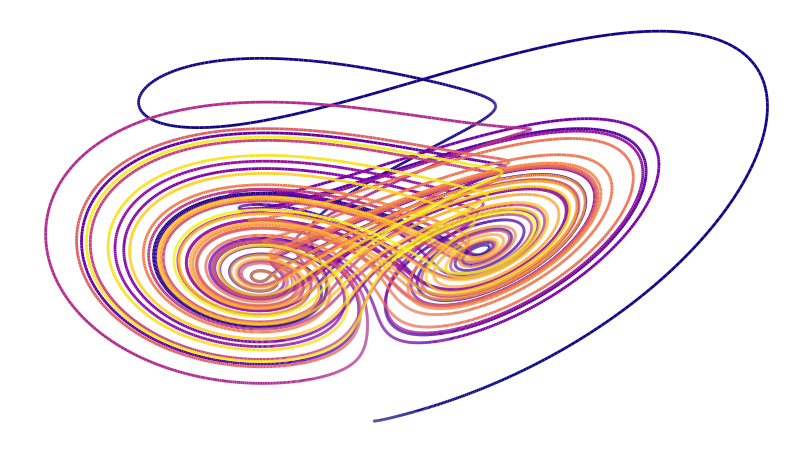
\includegraphics[scale=0.4]{graphics/attractor1.png}
		\\ {\small \caption{Chen attraktori Runge-Kutta menetelmällä}}
	\end{figure}
\end{frame}

\begin{frame}
    \frametitle{Sisältö}
    \begin{itemize}
    	\item{Yleistä ratkaisu menetelmistä}
    	\item{Menetelmien esittely}
    		\subitem{Euler}
    		\subitem{Runge-Kutta}
    		\subitem{Leapfrog}
    	\item{Menetelmien vertailu}
    	\item{Yhteenveto}
    \end{itemize}
	\begin{picture}(0, 0)
    	%\put(160, -135){\animategraphics[loop,controls,scale=0.5]{10}{graphics/content_sim-}{0}{16}}
    	\put(200, -30){\includegraphics[scale=0.17]{graphics/content_sim-80.png}}
    \end{picture}
\end{frame}

\begin{frame}
    \frametitle{Differentiaaliyhtälöt}

\end{frame}

\end{document}